\section{Suddivisione del lavoro}
Vengono qui di seguito descritti i ruoli ricoperti dai vari membri del gruppo durante lo svolgimento del progetto.
\subsection{\AR}
Nella fase di \AR{} ciascun componente dovrà ricoprire i seguenti ruoli e per la quantità di ore specificate:

\begin{table}[H]
	\centering
	\begin{tabular}{|l|c|c|c|c|c|c|c|}
		\hline
		\textbf{Nominativo} & 
		\multicolumn{6}{c|}{\textbf{Ore per ruolo}} & 
		\textbf{Ore totali} \\
		& Re & Am & An & Pj & Pr & Ve & \\
		\hline
		Nicola Dal Maso & & 7 & 10 & & & 10 & 27 \\
		Lorenzo Ferrarin & & 8 & 10 & & & 9 & 27 \\
		Beatrice Guerra & 15 & & 3 & & & 9 & 27 \\
		Marco Ponchia & & & 15 & & & 12 & 27 \\
		Tommaso Rosso & & 5 & 22 & & & & 27 \\
		Alice V. Sasso & & 9 & 18 & & & & 27 \\
		Mattia Zecchinato & 15 & & 12 & & & & 27 \\
		\hline
	\end{tabular}
	\caption{Ore per componente, fase di \AR{}}
\end{table}
I valori sono riassunti nel seguente grafico, che rappresenta in maniera visiva per quante ore un membro ricoprirà un determinato ruolo.
\begin{figure}[H]
	\centering
	\scalebox{0.6}{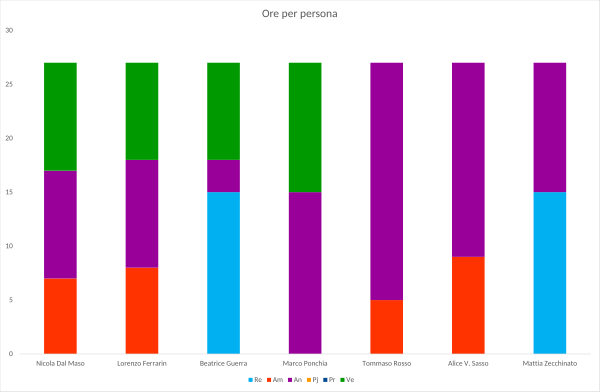
\includegraphics{img_suddlavoro/AA.png}}
	\caption{Ore per componente, fase di \AR{}}
\end{figure}


\subsection{\AD}
Nella fase di \AD{} ciascun componente dovrà ricoprire i seguenti ruoli e per la quantità di ore specificate:

\begin{table}[H]
	\centering
	\begin{tabular}{|l|c|c|c|c|c|c|c|}
		\hline
		\textbf{Nominativo} & 
		\multicolumn{6}{c|}{\textbf{Ore per ruolo}} & 
		\textbf{Ore totali} \\
		& Re & Am & An & Pj & Pr & Ve & \\
		\hline
		Nicola Dal Maso & & & 3 & & &  & 3 \\
		Lorenzo Ferrarin & & 1 & 2 & & &  & 3 \\
		Beatrice Guerra & & & 1 & & & 2 & 3 \\
		Marco Ponchia & & & 1 & & & 2 & 3 \\
		Tommaso Rosso & & 3 & & & & & 3 \\
		Alice V. Sasso & & & 3 & & & & 3 \\
		Mattia Zecchinato & 1 & & 2 & & & & 3 \\
		\hline
	\end{tabular}
	\caption{Ore per componente, fase di \AD}
\end{table}
I valori sono riassunti nel seguente grafico, che rappresenta in maniera visiva per quante ore un membro ricoprirà un determinato ruolo.
\begin{figure}[H]
	\centering
	\scalebox{0.6}{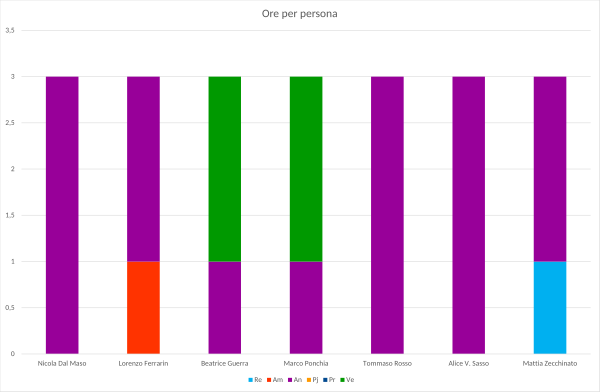
\includegraphics{img_suddlavoro/AD.png}}
	\caption{Ore per componente, fase di \AD{}}
\end{figure}

\subsection{\PA}
Nella fase di \PA{} ciascun componente dovrà ricoprire i seguenti ruoli e per la quantità di ore specificate:

\begin{table}[H]
	\centering
	\begin{tabular}{|l|c|c|c|c|c|c|c|}
		\hline
		\textbf{Nominativo} & 
		\multicolumn{6}{c|}{\textbf{Ore per ruolo}} & 
		\textbf{Ore totali} \\
		& Re & Am & An & Pj & Pr & Ve & \\
		\hline
		Nicola Dal Maso &4 & &3 &20 & & & 27 \\
		Lorenzo Ferrarin & & &2 &15 & &10 & 27 \\
		Beatrice Guerra & & &4 &14 & &10 & 28 \\
		Marco Ponchia & &4 &8 &15 & & & 27 \\
		Tommaso Rosso & &2 & &9 & &15 & 26 \\
		Alice V. Sasso &4 & &4 &20 & & & 28 \\
		Mattia Zecchinato & & &2 &8 & &20 & 30 \\
		\hline
	\end{tabular}
	\caption{Ore per componente, fase di \PA{}}
\end{table}
I valori sono riassunti nel seguente grafico, che rappresenta in maniera visiva per quante ore un membro ricoprirà un determinato ruolo.
\begin{figure}[H]
	\centering
	\scalebox{0.6}{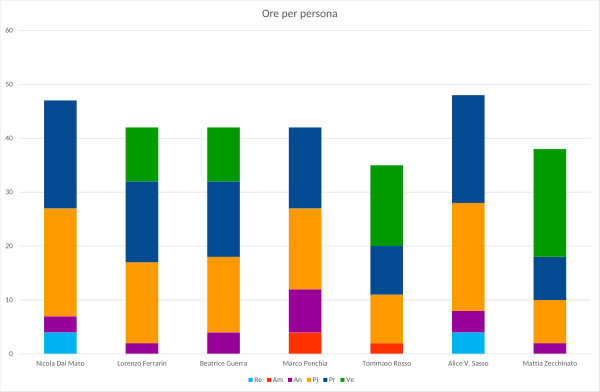
\includegraphics{img_suddlavoro/PA.png}}
	\caption{Ore per componente, fase di \PA{}}
\end{figure}

\subsection{\PD}
Nella fase di \PD{} ciascun componente dovrà ricoprire i seguenti ruoli e per la quantità di ore specificate:

\begin{table}[H]
	\centering
	\begin{tabular}{|l|c|c|c|c|c|c|c|}
		\hline
		\textbf{Nominativo} & 
		\multicolumn{6}{c|}{\textbf{Ore per ruolo}} & 
		\textbf{Ore totali} \\
		& Re & Am & An & Pj & Pr & Ve & \\
		\hline
		Nicola Dal Maso & & & &9 & &15 & 24 \\
		Lorenzo Ferrarin &5 & &2 &15 & & & 22 \\
		Beatrice Guerra & &4 & &18 & & & 22 \\
		Marco Ponchia &3 & & &18 & & & 21 \\
		Tommaso Rosso & & &2 &15 & &6 & 23 \\
		Alice V. Sasso & & & &6 & &15 & 21 \\
		Mattia Zecchinato & &4 & &17 & & & 21 \\
		\hline
	\end{tabular}
	\caption{Ore per componente, fase di \PD{}}
\end{table}
I valori sono riassunti nel seguente grafico, che rappresenta in maniera visiva per quante ore un membro ricoprirà un determinato ruolo.
\begin{figure}[H]
	\centering
	\scalebox{0.6}{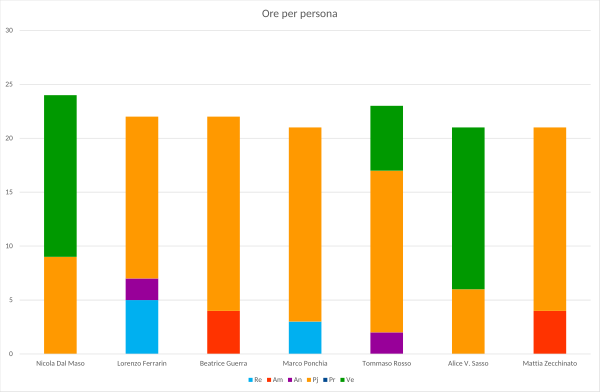
\includegraphics{img_suddlavoro/PD.png}}
	\caption{Ore per componente, fase di \PD{}}
\end{figure}

\subsection{\Cod}
Nella fase di \Cod{} ciascun componente dovrà ricoprire i seguenti ruoli e per la quantità di ore specificate:

\begin{table}[H]
	\centering
	\begin{tabular}{|l|c|c|c|c|c|c|c|}
		\hline
		\textbf{Nominativo} & 
		\multicolumn{6}{c|}{\textbf{Ore per ruolo}} & 
		\textbf{Ore totali} \\
		& Re & Am & An & Pj & Pr & Ve & \\
		\hline
		Nicola Dal Maso &4 & & & &25 & & 29 \\
		Lorenzo Ferrarin & & & &5 &23 &4 & 32 \\
		Beatrice Guerra & & & & &24 &7 & 31 \\
		Marco Ponchia & &4 & & &10 &18 & 32 \\
		Tommaso Rosso &5 & & &5 &23 & & 33 \\
		Alice V. Sasso & & & & &14 &18 & 32 \\
		Mattia Zecchinato & & & &5 &25 & & 30 \\
		\hline
	\end{tabular}
	\caption{Codifica}
\end{table}
I valori sono riassunti nel seguente grafico, che rappresenta in maniera visiva per quante ore un membro ricoprirà un determinato ruolo.
\begin{figure}[H]
	\centering
	\scalebox{0.6}{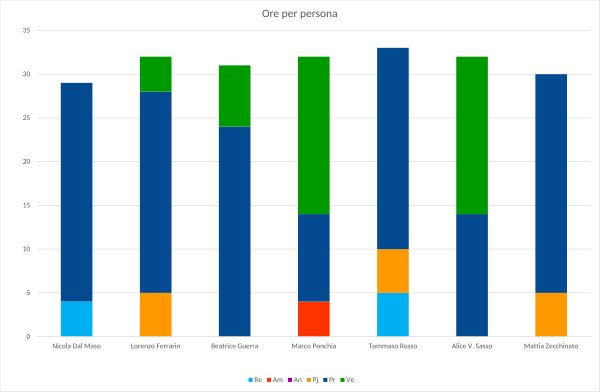
\includegraphics{img_suddlavoro/C.png}}
	\caption{Ore per componente, fase di \Cod{}}
\end{figure}

\subsection{\VV}
Nella fase di \VV{} ciascun componente dovrà ricoprire i seguenti ruoli e per la quantità di ore specificate:

\begin{table}[H]
	\centering
	\begin{tabular}{|l|c|c|c|c|c|c|c|}
		\hline
		\textbf{Nominativo} & 
		\multicolumn{6}{c|}{\textbf{Ore per ruolo}} & 
		\textbf{Ore totali} \\
		& Re & Am & An & Pj & Pr & Ve & \\
		\hline
		Nicola Dal Maso & &5 & &6 & &9 & 20 \\
		Lorenzo Ferrarin & &5 & &3 & &11 & 19 \\
		Beatrice Guerra &5 & & & & &14 & 19 \\
		Marco Ponchia & & & & &8 &12 & 20 \\
		Tommaso Rosso & & & &4 &4 &10 & 18 \\
		Alice V. Sasso & &6 & & & &13 & 19 \\
		Mattia Zecchinato &5 & & & & &14 & 19 \\
		\hline
	\end{tabular}
	\caption{Ore per componente, fase di \VV{}}
\end{table}
I valori sono riassunti nel seguente grafico, che rappresenta in maniera visiva per quante ore un membro ricoprirà un determinato ruolo.
\begin{figure}[H]
	\centering
	\scalebox{0.6}{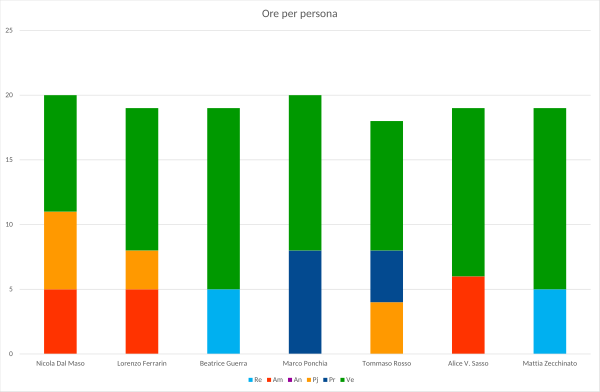
\includegraphics{img_suddlavoro/VV.png}}
	\caption{Ore per componente, fase di \VV{}}
\end{figure}

\subsection{Totale}
\subsubsection{Ore totali con investimento}
Le ore totali, comprese quelle investite in analisi, divise per componente durante il progetto saranno le seguenti:

\begin{table}[H]
	\centering
	\begin{tabular}{|l|c|c|c|c|c|c|c|}
		\hline
		\textbf{Nominativo} & 
		\multicolumn{6}{c|}{\textbf{Ore per ruolo}} & 
		\textbf{Ore totali} \\
		& Re & Am & An & Pj & Pr & Ve & \\
		\hline
		Nicola Dal Maso &8 &12 &16 &35 &25 &34 & 130 \\
		Lorenzo Ferrarin &5 &14 &16 &38 &23 &34 & 130 \\
		Beatrice Guerra &20 &4 &8 &32 &24 &42 & 130 \\
		Marco Ponchia &3 &8 &24 &33 &18 &44 & 130 \\
		Tommaso Rosso &5 &7 &27 &33 &27 &31 & 130 \\
		Alice V. Sasso &4 &15 &25 &26 &14 &46 & 130 \\
		Mattia Zecchinato &21 &4 &16 &30 &25 &34 & 130 \\
		\hline
	\end{tabular}
	\caption{Ore totali per componente compresa l'analisi non rendicontata}
\end{table}
%I valori sono riassunti nel seguente grafico, che rappresenta in maniera visiva per quante ore un membro ricoprirà un determinato ruolo.
%\begin{figure}[H]
%	\centering
%	\scalebox{0.6}{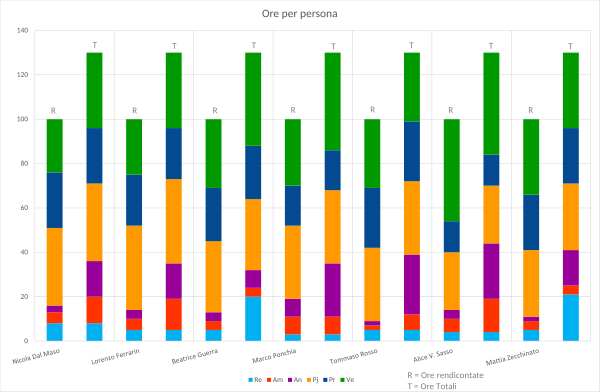
\includegraphics{img_suddlavoro/TOT.png}}
%	\caption{Ore totali per componente}
%\end{figure}

\subsubsection{Ore rendicontate}
Le ore totali rendicontate e divise per componente durante il progetto saranno le seguenti:

\begin{table}[H]
	\centering
	\begin{tabular}{|l|c|c|c|c|c|c|c|}
		\hline
		\textbf{Nominativo} & 
		\multicolumn{6}{c|}{\textbf{Ore per ruolo}} & 
		\textbf{Ore totali} \\
		& Re & Am & An & Pj & Pr & Ve & \\
		\hline
		Nicola Dal Maso &8 &5 &3 &35 &25 &24 & 100 \\
		Lorenzo Ferrarin &5 &5 &4 &38 &23 &25 & 100 \\
		Beatrice Guerra &5 &4 &4 &32 &24 &31 & 100 \\
		Marco Ponchia &3 &8 &8 &33 &18 &30 & 100 \\
		Tommaso Rosso &5 &2 &2 &33 &27 &31 & 100 \\
		Alice V. Sasso &4 &6 &4 &26 &14 &46 & 100 \\
		Mattia Zecchinato &5 &4 &2 &30 &25 &34 & 100 \\
		\hline
	\end{tabular}
	\caption{Ore totali rendicontate}
\end{table}
I valori sono riassunti nel seguente grafico, che rappresenta in maniera visiva per quante ore un membro ricoprirà un determinato ruolo.
\begin{figure}[H]
	\centering
	\scalebox{0.6}{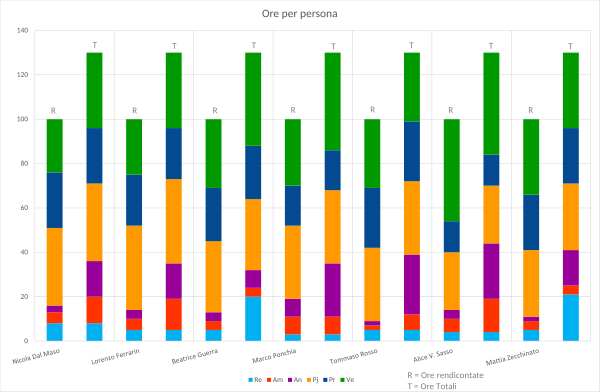
\includegraphics{img_suddlavoro/TOT.png}}
	\caption{Ore totali per componente}
\end{figure}





